\documentclass[letterpaper]{article}
\usepackage{aaai}
\usepackage{amsmath}
\usepackage{pgfplots}
\usepackage{caption}
\RequirePackage{booktabs}
\setlength{\pdfpagewidth}{8.5in} 
\setlength{\pdfpageheight}{11in}

\setcounter{secnumdepth}{0}
\pgfplotsset{compat=1.12}

\title{Automated Vacuum Cleaner Study}
\author{Rudra Sharma \and Joshua O'Dell \\ Colorado State University \\ Fort Collins, CO 80523 }
\begin{document}
\maketitle

\section{Introduction}

The purpose of this project is to simulate an automated vacuum cleaner (AUC). We represent a room as a 2D plane which has clean and dirty points/tiles. The goal of the vacuum cleaner is to clear all the dirty tiles and navigate/find a path around the the room.

In the project, we implement a variety of different vacuums and study their impact on performance. There have been several papers written on the study of automated vacuum cleaners. IRobot�s Roomba\cite{HSW_Roomba} is an example of such a robot, we will study this implementation when developing our own algorithms.

The paper \cite{Grid­based_Path­finding} explores a variety of grid based path finding algorithms, they identify an octet selection grid as an option of choosing the next point for the robot to move to as shown in figure 1. While the direct application of this paper will apply to room cleaning vacuums, these path-finding algorithms can be applied to robots searching for landmines, lawnmowers, and other agricultural tasks \cite{Optimal_Line­sweep­based}. 

The implementation for this project will be derived from a rudimentary implementation of a roomba robot \cite{Simulation_for_Roomba}. This implementation \cite{Simulation_for_Roomba} chooses its next tile based on a random selection from a 360$^{\circ}$ scale. We have instead opted to use the octet based selection as shown on figure 1 to choose the next tile. 

\begin{figure}[h]
\begin{center}
	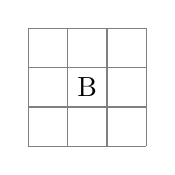
\begin{tikzpicture}
	\draw[step=.5cm,color=gray] (0,0) grid (1.5,1.5);
	\node at (+0.75,+0.75) {B};
	\end{tikzpicture}
\end{center}
\caption{ octet choice grid: the bot B has eight adjacent positions it can move to}
\label{figure:1}
\end{figure}
\section{Experiment Implementation}

The project implemented six distinct vacuum robots.  Each Robot has a different set of percepts, and the algorithm is adjusted to deal with it. The algorithms in each bot is a greedy algorithm with a different heuristic for calculating the cost based on the percepts it has. 

The following is a list of the capabilities of each Vacuum robot.
\begin{enumerate}  
\item \textbf{Preloaded Map:} Before the cleaning begins a map of the world is loaded into each the vacuum robot.  The robot also has knowledge of where it is on the map.
\item \textbf{Store explored tiles:} As the vacuum robot moves through the world it is allowed to store without limit, the tiles where it has been, and the status of that tile
\item \textbf{Proximity Sensor:} the vacuum robot has the ability to know when it is close to a wall.
\end{enumerate}  


\subsection{Random Bot}

\begin{tabular}{ r | l }  
	Preloaded map 		& No \\
	Store explored 		& No \\
	Proximity 		 	& No \\
	sensor 					 \\
\end{tabular}
\quad
\begin{tabular}{ r | l }  
	Observable		& Unobservable 	\\
	Deterministic	& Deterministic \\
	Episodic		& Sequential	\\
	Static		 	& Static 		\\
	Discrete 		& Discrete 		\\
	Agents		 	& Single 		\\
\end{tabular}
The Random robot was the first Robot we implemented for our study. This robot has no form of storage or sensors to guide it in cleaning a room. 
When the robot is initialized, it will clean the location it is placed on and then it will randomly select a next point based on what is adjacent to it, thereby giving it eight options. See figure 1 for display of the octet grid selection for the random robot. 



\subsection{Store Map Bot}

\begin{tabular}{ r | l }  
	Preloaded Map 		& Yes \\
	Store explored 		& No \\
	Proximity  		 	& No \\
	sensor 					 \\
\end{tabular}
\quad
\begin{tabular}{ r | l }  
	Observable 		& Fully 		\\
	Deterministic 	& Deterministic \\
	Episodic		& Sequential	\\
	Static		 	& Static 		\\
	Discrete 		& Discrete 		\\
	Agents		 	& Single 		\\	
\end{tabular}
The store map was a Robot which was given the the exact boundaries of the room prior to start. The objective of this robot was to use its knowledge of the boundaries of the room to avoid attempting to go outside the boundaries of the room. This robot was an extension to the random robot so the path that it choose next was also a random selection from the octet grid, however it knows to avoid the points which represent tiles outside the boundaries of the room.

\subsection{Store Map with Direction Bot}
\begin{tabular}{ r | l }  
	Preloaded Map 		& Yes \\
	Store explored		& No \\
	Proximity 		 	& No \\
	sensor 					 \\
\end{tabular}
\quad
\begin{tabular}{ r | l }  
	Observable		& Fully 		\\
	Deterministic	& Deterministic \\
	Episodic		& Sequential	\\
	Static		 	& Static 		\\
	Discrete 		& Discrete 		\\
	Agents		 	& Single 		\\	
\end{tabular}
The store map with direction was an extension to the store map. However, this bot does not randomly select its next tile in the room. Instead it uses a strategy of maintaining a direction until it reaches the boundary of a room. After it reaches a boundary it will slide to the adjacent side and do a 180$^{\circ}$ turn and travel in the the opposite direction it came from until it hits the opposite boundary of the room. It will keep repeating this process until it completes the entire room.

\subsection{Proximity Bot}

\begin{tabular}{ r | l }  
	Preloaded Map 		& No \\
	Store Explored 		& No \\
	Proximity  		 	& Yes \\
	sensor 					 \\
\end{tabular}
\quad
\begin{tabular}{ r | l }  
	Observable		& Partially		\\
	Deterministic	& Deterministic \\
	Episodic		& Sequential 	\\
	Static		 	& Static 		\\
	Discrete 		& Discrete 		\\
	Agents		 	& Single 		\\	
\end{tabular} 
 	
 		
 		
This program was implemented by mimicking the `Roomba''s algorithm \cite{HSW_Roomba}.  The algorithm creates a spiral from the starting position outward.  Once the proximity sensor detects a wall the algorithm changes.  The new algorithm will choose a random direction, and continue straight along that direction until the proximity sensor detects another wall, at which point another random direction is chosen.  

The largest hurdle with this program was finding the best equation to calculate a spiral.  At each step in the simulation a new direction was calculated using the following equation.
$ 22.5 - (\mathrm {e} ^ x * 45)$
where time x was decremented by $0.01$ during each step.  The program appeared to be efficient, however when run, we saw that it had difficulty achieving 10\% coverage in a timely manner.  We attribute this to some tweaking that is necessary on the spiral formula.  We believe it is going over the same places too much, however given our grid approach more aggressive spiraling would result in a missed grid tile in the center.


\subsection{Stored Explored Bot}

\begin{tabular}{ r | l }  
	Preloaded Map 		& No \\
	Store explored 		& Yes \\
	Proximity 		 	& No \\
	sensor 					 \\
\end{tabular}
\quad
\begin{tabular}{ r | l }  
	Observable 		& Unobservable 	\\
	Deterministic 	& Deterministic \\
	Episodic		& Sequential	\\
	Static		 	& Static 		\\
	Discrete 		& Discrete 		\\
	Agents		 	& Single 		\\	
\end{tabular}
This program is allowed to maintain a list of the grid tiles where it has visited.  It is allowed to know where each of these grid tiles are in relation to its current location.
The algorithm used in this program will attempt keep the vacuum close to the grid tiles that were previously visited.  To do this the following steps are taken.  
\begin{enumerate}  
\item Get a list of all the possible steps we can take.
\item For each step determine a ranking.  This is calculated by summing the distance to each of the existing items.
\item Choose the step with the lowest rank.
\end{enumerate}

If a spot is chosen that is outside of the grid, the program's time complexity ranking is incremented, however the robot will not be able to move there.  We also try to avoid revisiting grid tiles that have already been visited.  To do this, if a possible location turns up in our visited locations, then we increase the rank.  Essentially moving the rank high enough that other options, even if they move away from the existing cluster, will be chosen.  Thus, the rank equation is as follows.
\[
  Rank=
	\begin{cases}
		visited=False: \sum{distance(visited)}\\
		visited=True: sizeOf(Visited)
	\end{cases}
\]

\subsection{Store Explored + Proximity Bot}

\begin{tabular}{ r | l }  
	Preloaded Map 		& No \\
	Store explored 		& Yes \\
	Proximity 		 	& Yes \\
	sensor 					 \\
\end{tabular}
\quad
\begin{tabular}{ r | l }  
	Observable		& Partially 	\\
	Deterministic	& Deterministic	\\
	Episodic		& Sequential	\\
	Static		 	& Static 		\\
	Discrete 		& Discrete 		\\
	Agents		 	& Single 		\\	
\end{tabular}
This program is an extension of the `store explored' program.  An observation we made about the store explored was that depending on where it started, we could get into a situation where we had finished the middle of the room, and one side, but needed to complete the other side.  To resolve this we have to cross the already cleaned region, which our algorithm did not handle elegantly.

Adding a proximity sensor to the vacuum robot allowed us to do the following.  When the robot first starts cleaning it chooses a single direction.  Once it reaches a wall it then begins the existing algorithm from the `store explored' robot.  Then this robot can start cleaning on one side of the room, and not have to back track.  

\section{Results}
\subsection{Experiment 1}
We began our data gathering by running each robot and asking it to clean a certain percentage of the room.  The Robot was given 1,000,000 steps to complete the task.  Table:\ref{table:1} describes our results of this initial experiment.  

\begin{table}
\begin{tabular}{ r | l l l l l }  
					& 10\%		& 50\%		& 80\%		& 100\%		\\
	\midrule
	Random			& 96\% 		& 77\% 		& 40\%		& 12\%		\\
	Store Map		& 100\%		& 100\% 	& 100\%  	& 100\% 	\\
	Store Map 		& 100\%		& 100\% 	& 100\%  	& 100\% 	\\
	with direction \\
	Proximity		& 40\%		& 34\% 		& 27\%  	& 25\% 		\\
	Store Explored 	& 100\%		& 100\% 	& 100\%  	& 100\% 	\\
	Store Explored 	& 100\%		& 100\% 	& 100\%  	& 100\% 	\\
	with proximity 	\\
\end{tabular}
\caption[success]{Percent success (depth = 1,000,000)}
\label{table:1}
\end{table}

\begin{figure}
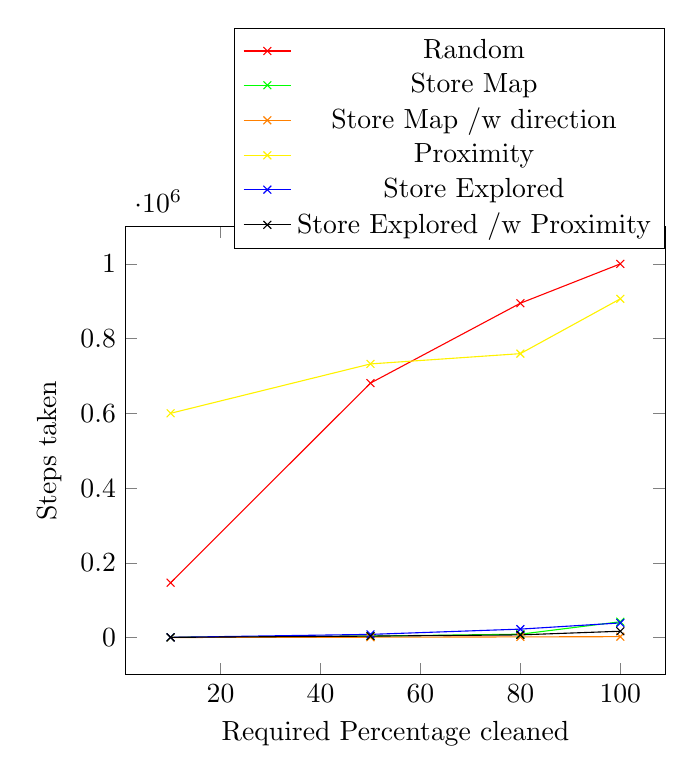
\begin{tikzpicture}
	\begin{axis}[
		xlabel=Required Percentage cleaned,
		ylabel=Steps taken,
		legend style={at={(1.0,0.95)},anchor=south east}]
	\addplot[color=red,mark=x] coordinates {
 		(  10,   146783)
 		(  50,   680976)
 		(  80,   894746)
 		( 100,  1000000)
	};
	\addlegendentry{Random}
	\addplot[color=green,mark=x] coordinates {
 		(  10,   373)
 		(  50,  3895)
 		(  80,  9006)
 		( 100, 42284)
	};
	\addlegendentry{Store Map}
	\addplot[color=orange,mark=x] coordinates {
 		(  10,   160)
 		(  50,   947)
 		(  80,  1756)
 		( 100,  2408)
	};
	\addlegendentry{Store Map /w direction}
	\addplot[color=yellow,mark=x] coordinates {
 		(  10,  600159)
 		(  50,  732261)
 		(  80,  759790)
 		( 100,  906491)
	};
	\addlegendentry{Proximity}
	\addplot[color=blue,mark=x] coordinates {
 		(  10,    535)
 		(  50,   8491)
 		(  80,  22586)
 		( 100,  39161)
	};
	\addlegendentry{Store Explored}
	\addplot[color=black,mark=x] coordinates {
 		(  10,    539)
 		(  50,   3857)
 		(  80,   7163)
 		( 100,  16898)
	};
	\addlegendentry{Store Explored /w Proximity}
	\end{axis}
\end{tikzpicture}
\caption{Steps taken by each Robot to complete the required percentage (depth = 1,000,000)}
\label{figure:2}
\end{figure}

The results of this experiment show us that at 1,000,000 steps most of the robots can succeed even if the requirement is to clean 100\% of the room.  However, the above table hides a key element, `how long did it actually take'.  Table:\ref{table:2} shows in more detail how many iterations each robot actually took to complete the task.  The numbers provided are an average of 100 runs, this average includes the failures and successes.  If a robot was unable to complete the task then its step count would reach 1,000,000 and halt, indicating failure to achieve coverage, and contribute to bringing the average processing steps higher.  Figure:\ref{figure:2} shows this in a graphical format.  We can see that the Random and Proximity robots initially took the longest to complete their tasks, and continued to do so as the required percentage increased.  

\begin{table}
\begin{tabular}{ r | l l l l l }  
					& 10\%		& 50\%		& 80\%		& 100\%		\\
	\midrule
	Random			& 146783 	& 680976 	& 894746 	& 1000000	\\
	Store Map		& 373		& 3895 		& 9006  	& 42284 	\\
	Store Map 		& 160		& 947 		& 1756 		& 2408		\\
	with direction \\
	Proximity		& 600159	& 732261 	& 759790 	& 906491	\\
	Store Explored 	& 535		& 8491		& 22586		& 39161		\\
	Store Explored 	& 539		& 3857 		& 7163 		& 16898		\\	
	with proximity 	\\
\end{tabular}
\caption{Actual steps taken to complete task (depth = 1,000,000)}
\label{table:2}
\end{table}

\subsection{Experiment 2}
1,000,000 iterations of the program may not be an acceptable amount of time for a robot to clean a room.  If we assume that it takes one second for a robot to clean a square and move on, then each robot would take close to $ 1000000 / 60 / 60 / 24 = 11.5 days $ to complete it's task. 

Our second experiment took this into account and lowered the maximum steps to 10,000.  Table:\ref{table:3} shows the outcome of this, and Figure:\ref{figure:3} shows this graphically.  

\begin{table}[!ht]
\begin{tabular}{ r | l l l l l }  
					& 10\%		& 50\%		& 80\%		& 100\%		\\
	\midrule
	Random			& 96\% 		& 77\% 		& 40\%		& 12\%		\\
	Store Map		& 100\%		& 100\% 	& 100\%  	& 100\% 	\\
	Store Map 		& 100\%		& 100\% 	& 100\%  	& 100\% 	\\
	with direction \\
	Proximity		& 40\%		& 34\% 		& 27\%  	& 25\% 		\\
	Store Explored 	& 100\%		& 100\% 	& 100\%  	& 100\% 	\\
	Store Explored 	& 100\%		& 100\% 	& 100\%  	& 100\% 	\\
	with proximity 	\\
\end{tabular}
\caption[success]{Percent success (depth = 1,000,000)}
\label{table:3}
\end{table}

\begin{figure}
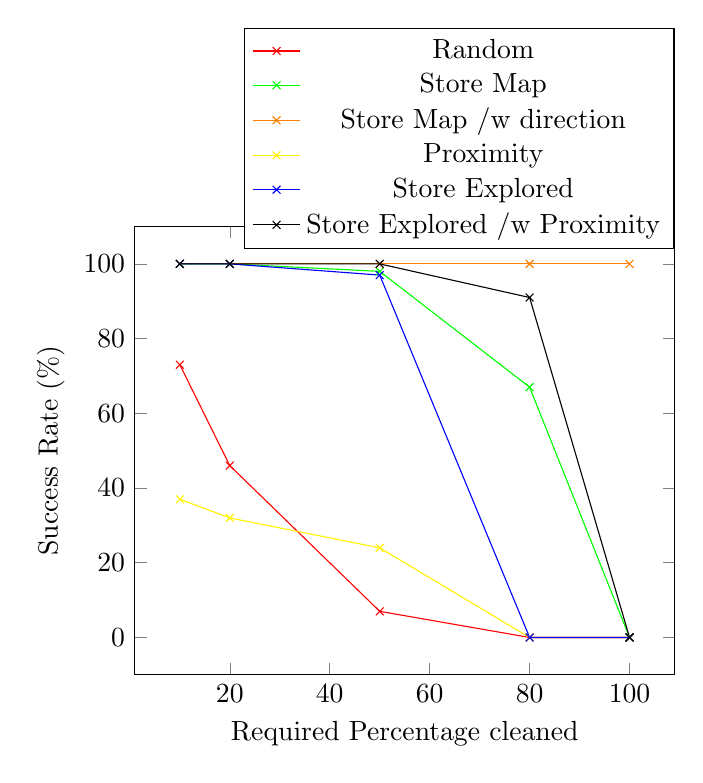
\begin{tikzpicture}
	\begin{axis}[
		xlabel=Required Percentage cleaned,
		ylabel=Success Rate (\%),
		legend style={at={(1.0,0.95)},anchor=south east}]
	\addplot[color=red,mark=x] coordinates {
 		(  10, 73)
 		(  20, 46)
 		(  50,  7)
 		(  80,  0)
 		( 100,  0)
	};
	\addlegendentry{Random}
	\addplot[color=green,mark=x] coordinates {
 		(  10, 100)
 		(  20, 100)
 		(  50,  98)
 		(  80,  67)
 		( 100,   0)
	};
	\addlegendentry{Store Map}
	\addplot[color=orange,mark=x] coordinates {
 		(  10,  100)
 		(  20,  100)
 		(  50,  100)
 		(  80,  100)
 		( 100,  100)
	};
	\addlegendentry{Store Map /w direction}
	\addplot[color=yellow,mark=x] coordinates {
 		(  10, 37)
 		(  20, 32)
 		(  50, 24)
 		(  80,  0)
 		( 100,  0)
	};
	\addlegendentry{Proximity}
	\addplot[color=blue,mark=x] coordinates {
 		(  10, 100)
 		(  20, 100)
 		(  50,  97)
 		(  80,   0)
 		( 100,   0)
	};
	\addlegendentry{Store Explored}
	\addplot[color=black,mark=x] coordinates {
 		(  10,  100)
 		(  20,  100)
 		(  50,  100)
 		(  80,   91)
 		( 100,   0)
	};
	\addlegendentry{Store Explored /w Proximity}
	\end{axis}
\end{tikzpicture}
\caption{Percentage of successful runs (depth = 10,000)}
\label{figure:3}
\end{figure}

\begin{table}
\begin{tabular}{ r | l l l l l }  
					& 10\%		& 50\%		& 80\%		& 100\%		\\
	\midrule
	Random			& 3570 		& 9752 		& 10000 	& 10000	\\
	Store Map		& 375		& 3941 		& 7905  	& 10000 	\\
	Store Map 		& 160		& 588 		& 1707 		& 2403		\\
	with direction \\
	Proximity		& 6431		& 9476 		& 10000 	& 10000		\\
	Store Explored 	& 520		& 8539		& 10000		& 10000		\\
	Store Explored 	& 533		& 3864 		& 6924 		& 10000		\\	
	with proximity 	\\
\end{tabular}
\caption{Actual steps taken to complete task (depth = 10,000)}
\label{table:4}
\end{table}

\begin{figure}
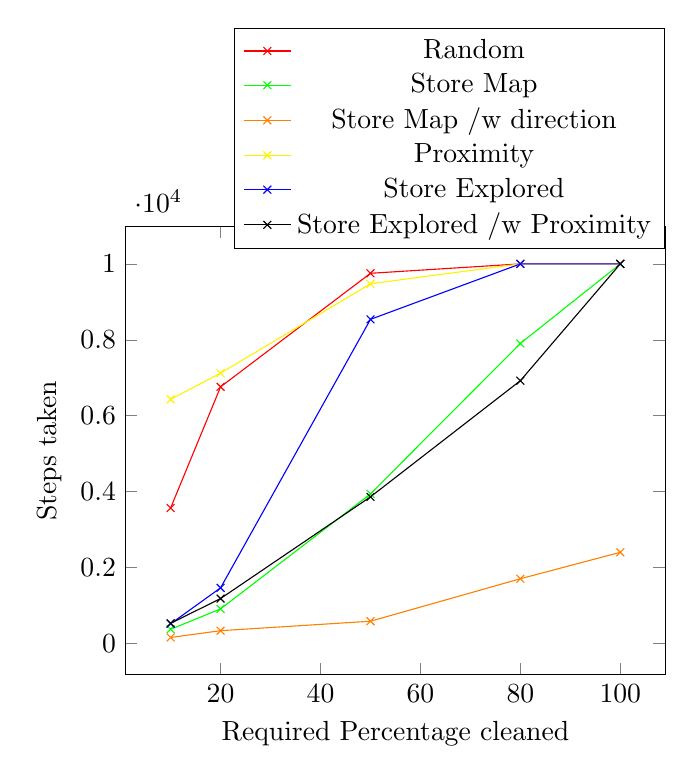
\begin{tikzpicture}
	\begin{axis}[
		xlabel=Required Percentage cleaned,
		ylabel=Steps taken,
		legend style={at={(1.0,0.95)},anchor=south east}]
	\addplot[color=red,mark=x] coordinates {
 		(  10,   3570)
 		(  20,   6761)
 		(  50,   9752)
 		(  80,  10000)
 		( 100,  10000)
	};
	\addlegendentry{Random}
	\addplot[color=green,mark=x] coordinates {
 		(  10,   375)
 		(  20,   913)
 		(  50,  3941)
 		(  80,  7905)
 		( 100, 10000)
	};
	\addlegendentry{Store Map}
	\addplot[color=orange,mark=x] coordinates {
 		(  10,   160)
 		(  20,   339)
 		(  50,   588)
 		(  80,  1707)
 		( 100,  2403)
	};
	\addlegendentry{Store Map /w direction}
	\addplot[color=yellow,mark=x] coordinates {
 		(  10,   6431)
 		(  20,   7123)
 		(  50,   9476)
 		(  80,  10000)
 		( 100,  10000)
	};
	\addlegendentry{Proximity}
	\addplot[color=blue,mark=x] coordinates {
 		(  10,    520)
 		(  20,   1467)
 		(  50,   8539)
 		(  80,  10000)
 		( 100,  10000)
	};
	\addlegendentry{Store Explored}
	\addplot[color=black,mark=x] coordinates {
 		(  10,    533)
 		(  20,   1185)
 		(  50,   3864)
 		(  80,   6924)
 		( 100,  10000)
	};
	\addlegendentry{Store Explored /w Proximity}
	\end{axis}

\end{tikzpicture}
\caption{Steps taken by each Robot to complete the required percentage (depth = 10,000)}
\label{figure:4}
\end{figure}

In this experiment we can see more clearly that most of the robots can complete the task when only a small percentage of the room is required.  However, when the coverage percentage increases most robots have fewer successful runs.  We see that the `Random' and `Proximity' Robots do not do a very good job once they are required to clean more then half of the room.  The `Stored Map w/ Direction' always completes the task, and the `Store Explored w/ Proximity' does a great job until it is required to clean the entire room.

\subsection{Experiment 3}
Running a slightly different experiment we tested to see how close some of these robots came to succeeding when asked to clean the whole room.  Table:\ref{table:5} shows the results of this experiment. The interesting thing to note here is that while `Store Map' and `Store Explored with Proximity' did not complete 100\% of the room they got very close at 82\% and 94\% respectively.  

\begin{table}
\begin{tabular}{ r | l l l l l }  
									& \% cleaned \\
	\midrule
	Random							& 24 	\\
	Store Map						& 82	\\
	Store Map with direction		& 100	\\
	Proximity						& 17 	\\
	Store Explored 					& 54	\\
	Store Explored with proximity	& 94	\\	
\end{tabular}
\caption{Actual percentage cleaned (depth = 10,000)}
\label{table:5}
\end{table}

\section{Conclusion}

One of the questions we had when we started this project was `Can a crippled robot perform as well as an Omnipotent one'?  The answer we found out was absolutely not.  However given some clever algorithms and relaxing the requirements of 100\% clean allows for these robots to do `OK'.  When the robot is given the map of the world, and knows where it is, then it is easy to come up with a very efficient algorithm to clean every part of the room.  However when we removed this ability the results got quite a bit worse.  That being said the `Store Explored with Proximity' did very well on its own.  However, the realization of this robot may not be as realistic as we might hope.  Being able to store all the places where the robot has been could be difficult to implement outside of a simulation.

The commercial product most known in this area is the `Roomba.'  The Roomba's algorithm\cite{HSW_Roomba} is similar to the `Proximity' one that we implemented.  We found that this algorithm is pretty inefficient,  However we were hard pressed to find a better one given the limited percepts.  I also believe that this algorithm performs better when measured in a non grid environment.  Given the spiral nature of the algorithm it was difficult to map that onto a grid without missing grid positions, or going over them more then once.  This robot has no knowledge of where it is or where it has been, it simply switches between two different algorithms based on whether it has hit a wall yet.

There is still a lot of room in this field for better algorithms.  Since we have found that knowledge of the room makes a huge difference in finding an efficient path, perhaps a learning robot could be created.  One that uses the percepts it has to create a statistical probability of where it is in the room based on the given percepts.  We will leave this investigation to future projects. 

% \cite[p. 2] {Optimized_Path_Planning}
\nocite{*}
\bibliography{report}
\bibliographystyle{aaai}
\end{document}


